\section{Основная часть}

\subsection{Постановка задачи}

Необходимо разработать метод определения переменного ритма и переменного темпа музыки на основе байесовского иерархического моделирования. Для этого требуется составить модели, которые будут использовать статистические данные о музыке, такие как темп и тактовый размер. Модель для определения темпа должна также учитывать жанр анализируемой музыки. Составленные модели должны быть обучены на наборе данных, включающих в том числе различные жанры~\cite{dataset}. После обучения моделей, они должны быть протестированы на новых данных, чтобы оценить их точность и эффективность.

Входные данные:

\begin{itemize}
	\item[---] аудиофайл;
	\item[---] жанр музыки (строка).
\end{itemize}

Выходные данные:

\begin{itemize}
	\item[---] набор темпов (целые числа, в BPM);
	\item[---] набор тактовых размеров (обыкновенные дроби в формате <<a/b>>).
\end{itemize}

Оба набора выходных данных должны сопровождаться временем, соответствующим каждому темпу или размеру.

Ограничения:

\begin{itemize}
	\item[---] загружаемые аудиофайлы должны быть в формате mp3;
	\item[---] знаменатель тактового размера принимается равным 4.
\end{itemize}

\subsection{Этапы работы метода}

\subsubsection{Определение темпа}

Ниже представлены IDEF0-диаграммы для алгоритма определения переменного темпа музыки~\cite{kubler_pymc3,bayesian}.

\begin{figure}[h]
	\centering
	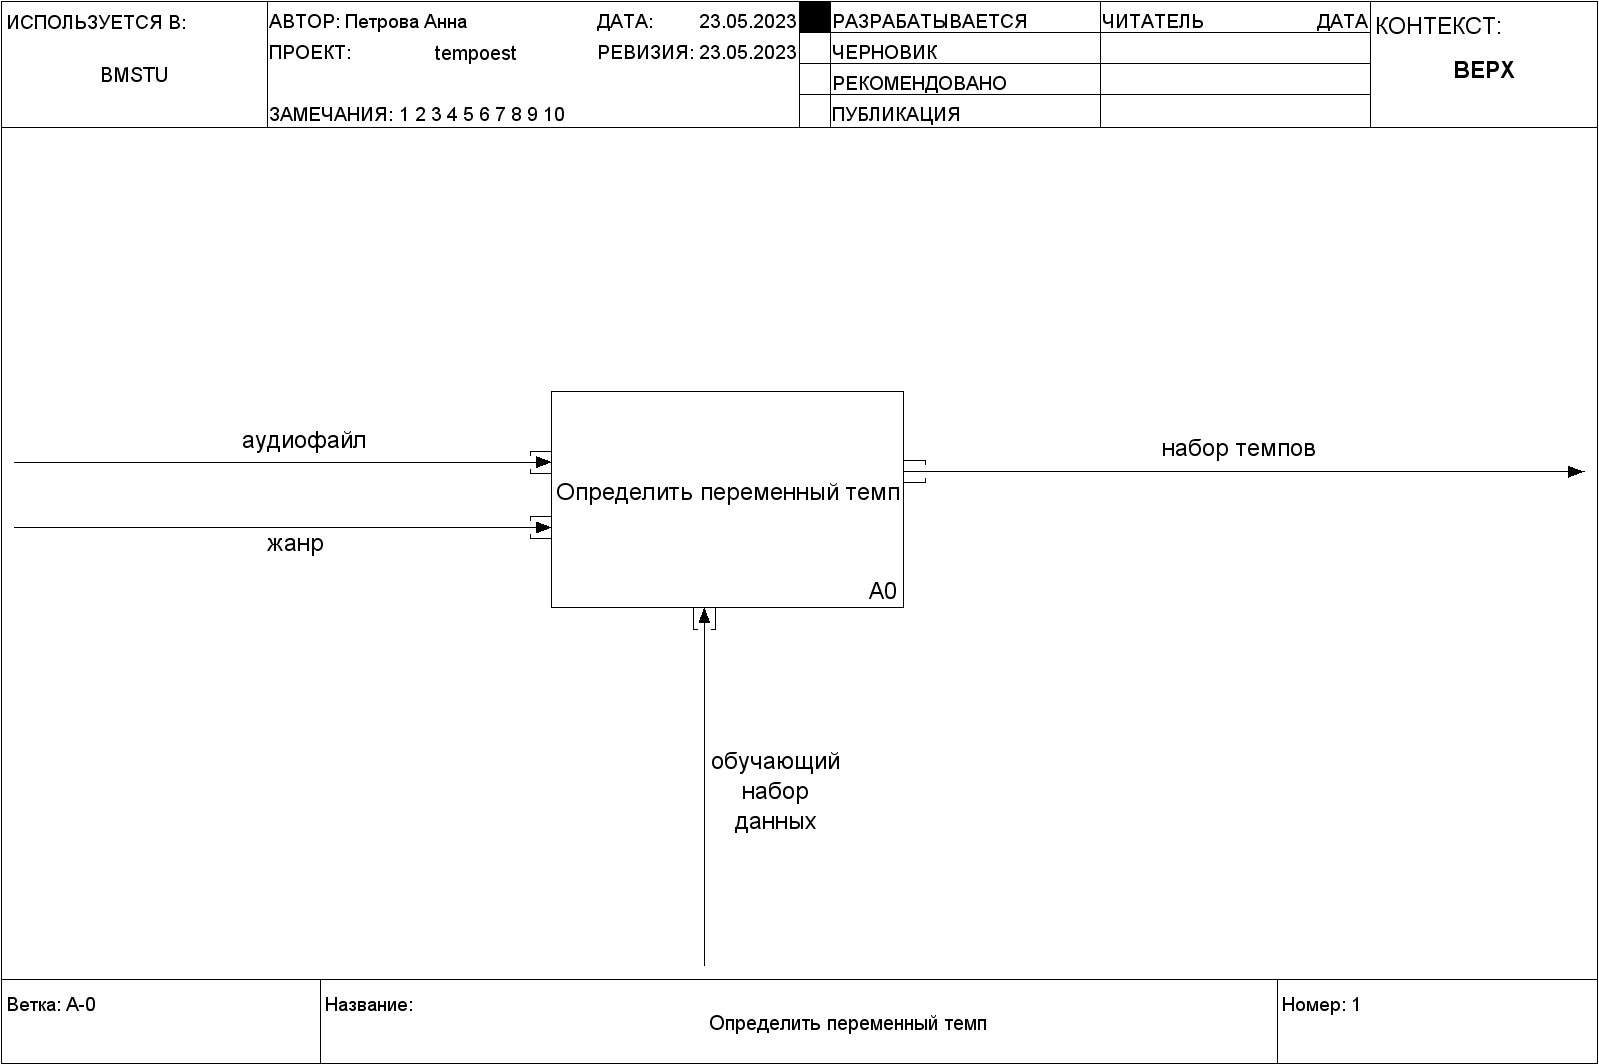
\includegraphics[scale=0.25]{inc/img/tempo_idef/01_A-0.png}
	\caption{IDEF0 нулевого уровня}
	\label{img:tempo_0}
\end{figure}

\begin{figure}[h]
	\centering
	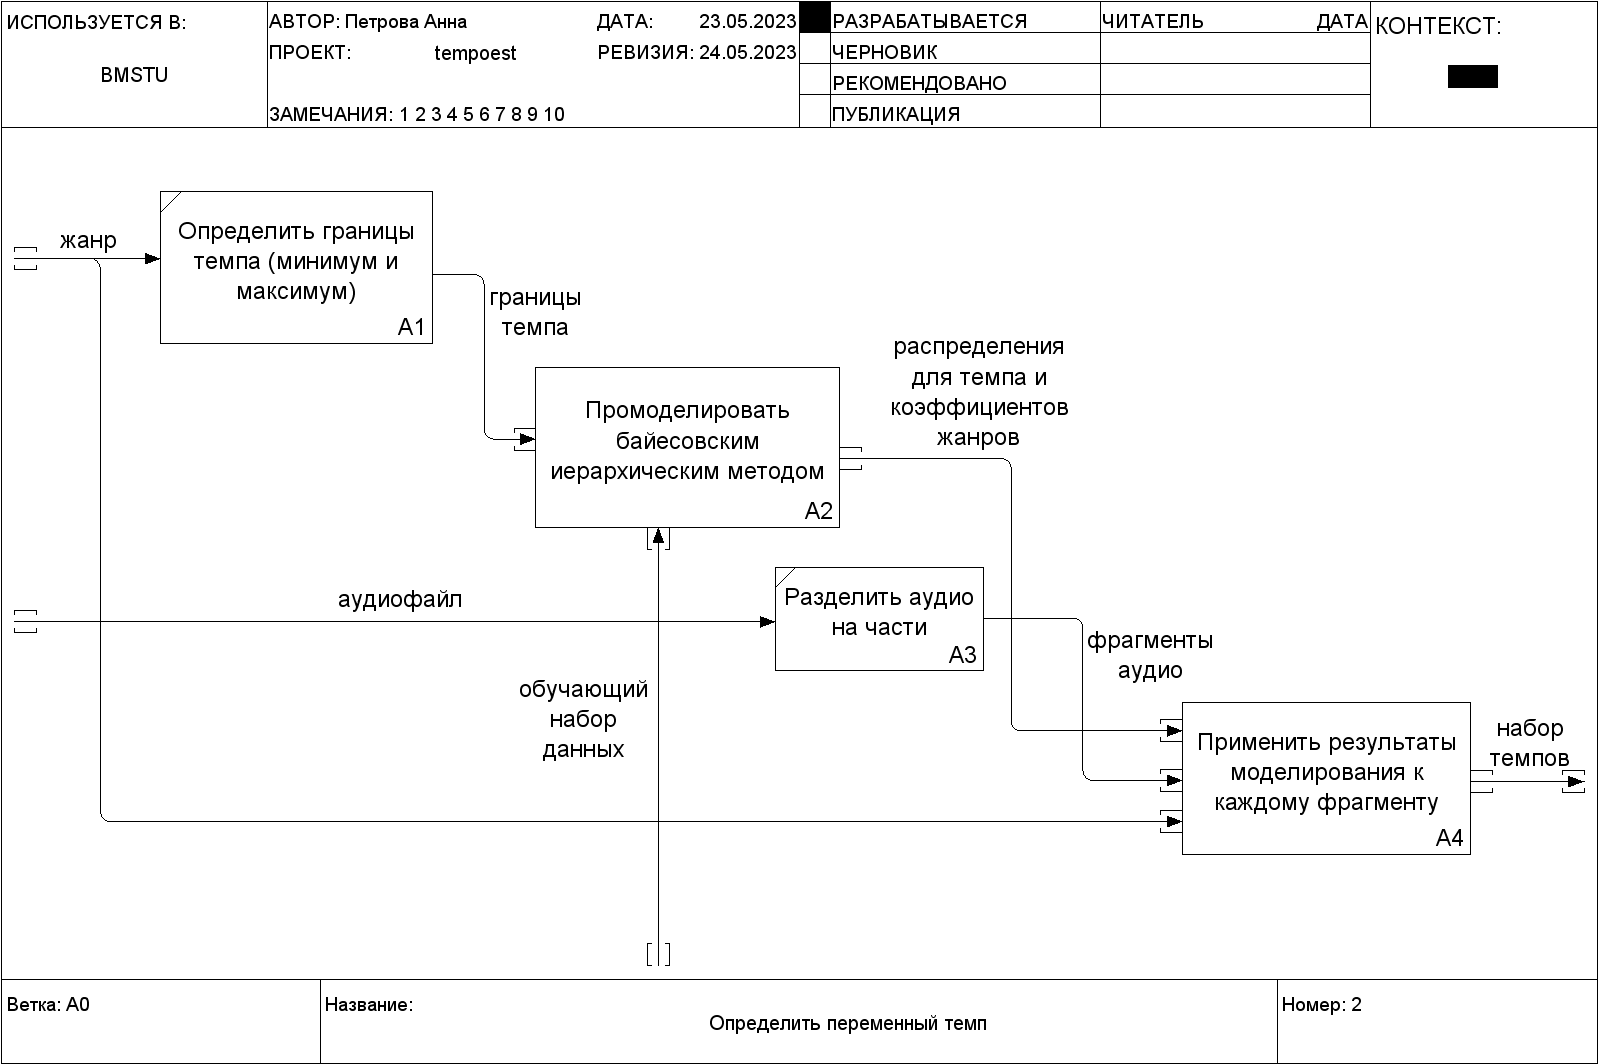
\includegraphics[scale=0.25]{inc/img/tempo_idef/02_A0.png}
	\caption{Определение переменного темпа}
	\label{img:tempo_1}
\end{figure}

\begin{figure}[h]
	\centering
	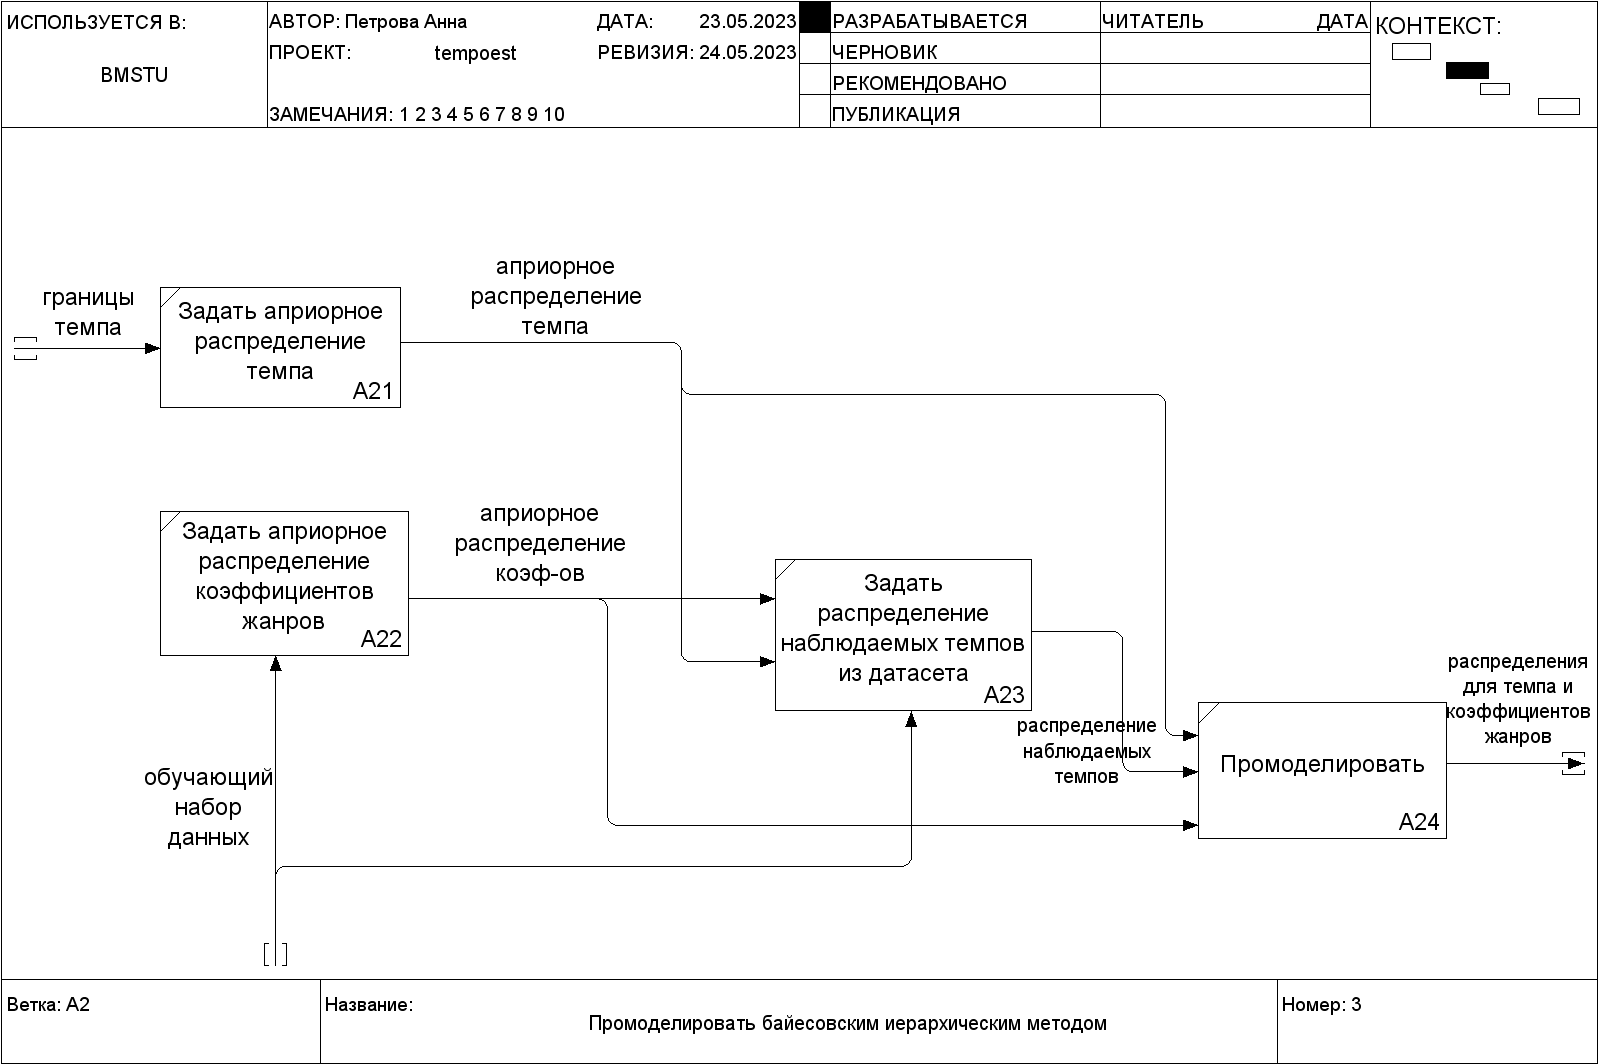
\includegraphics[scale=0.25]{inc/img/tempo_idef/03_A2.png}
	\caption{Байесовское моделирование}
	\label{img:tempo_2}
\end{figure}

\begin{figure}[h]
	\centering
	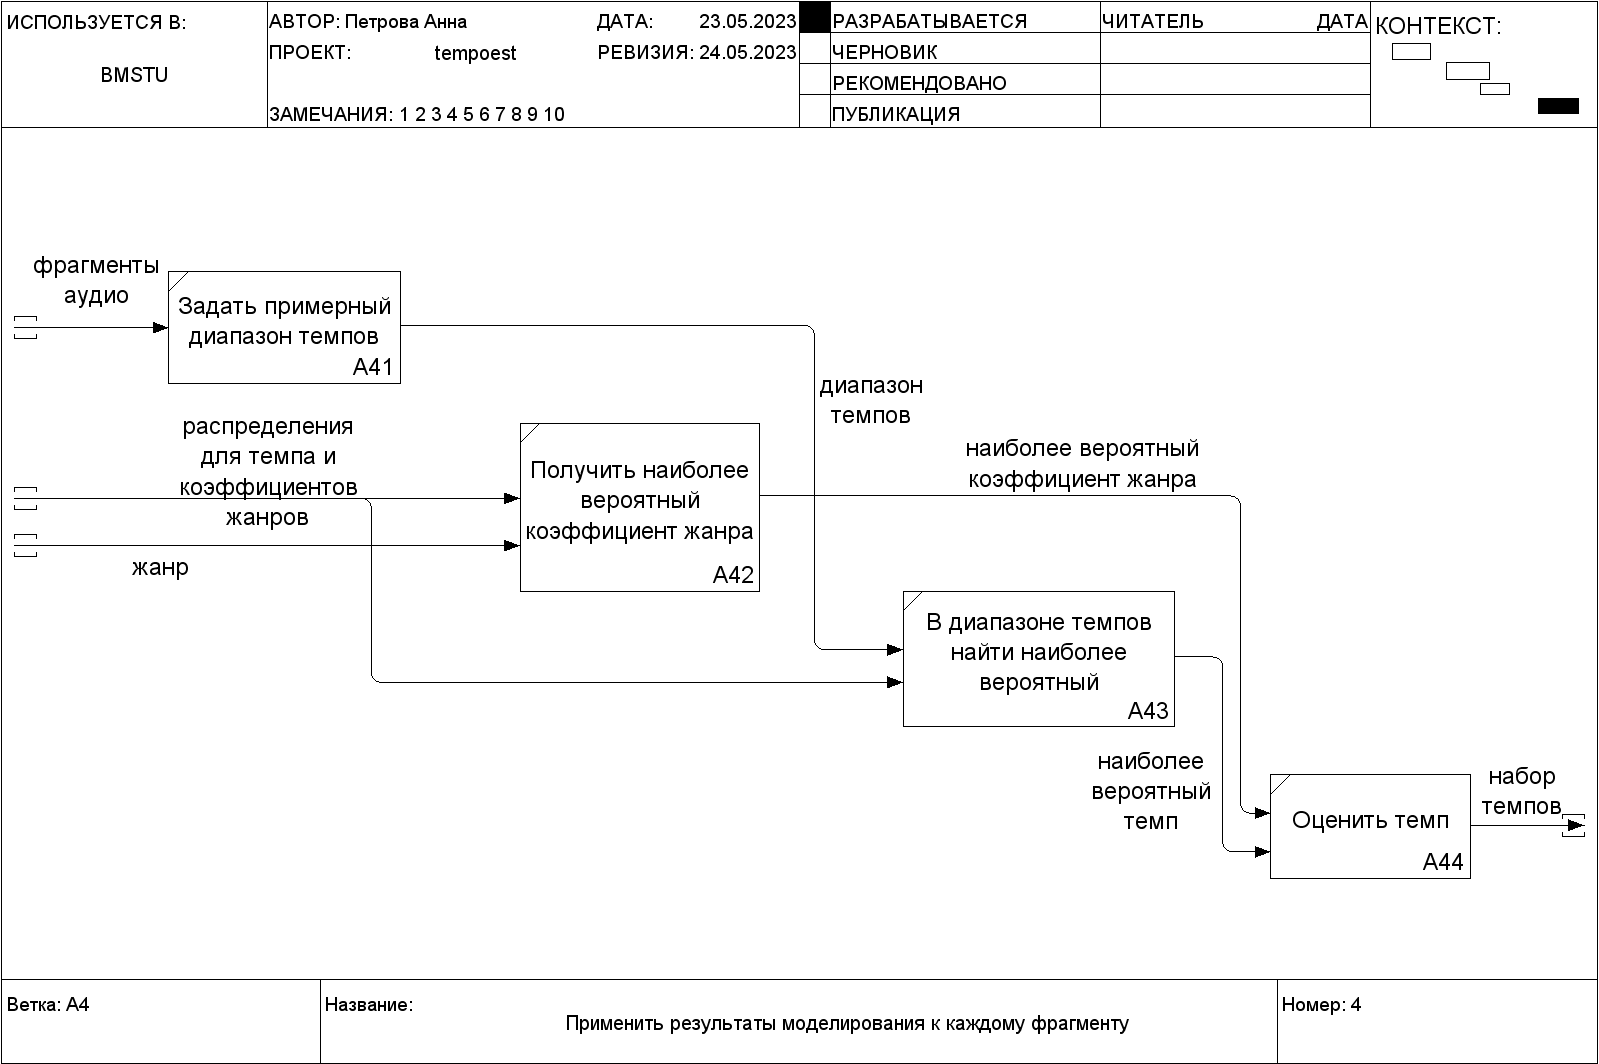
\includegraphics[scale=0.25]{inc/img/tempo_idef/04_A4.png}
	\caption{Применение результатов к фрагментам аудио}
	\label{img:tempo_3}
\end{figure}

\clearpage

\subsubsection{Определение ритма}

Ниже приведены IDEF0-диаграммы для алгоритма определения переменного ритма (тактового размера) музыки.

\begin{figure}[h]
	\centering
	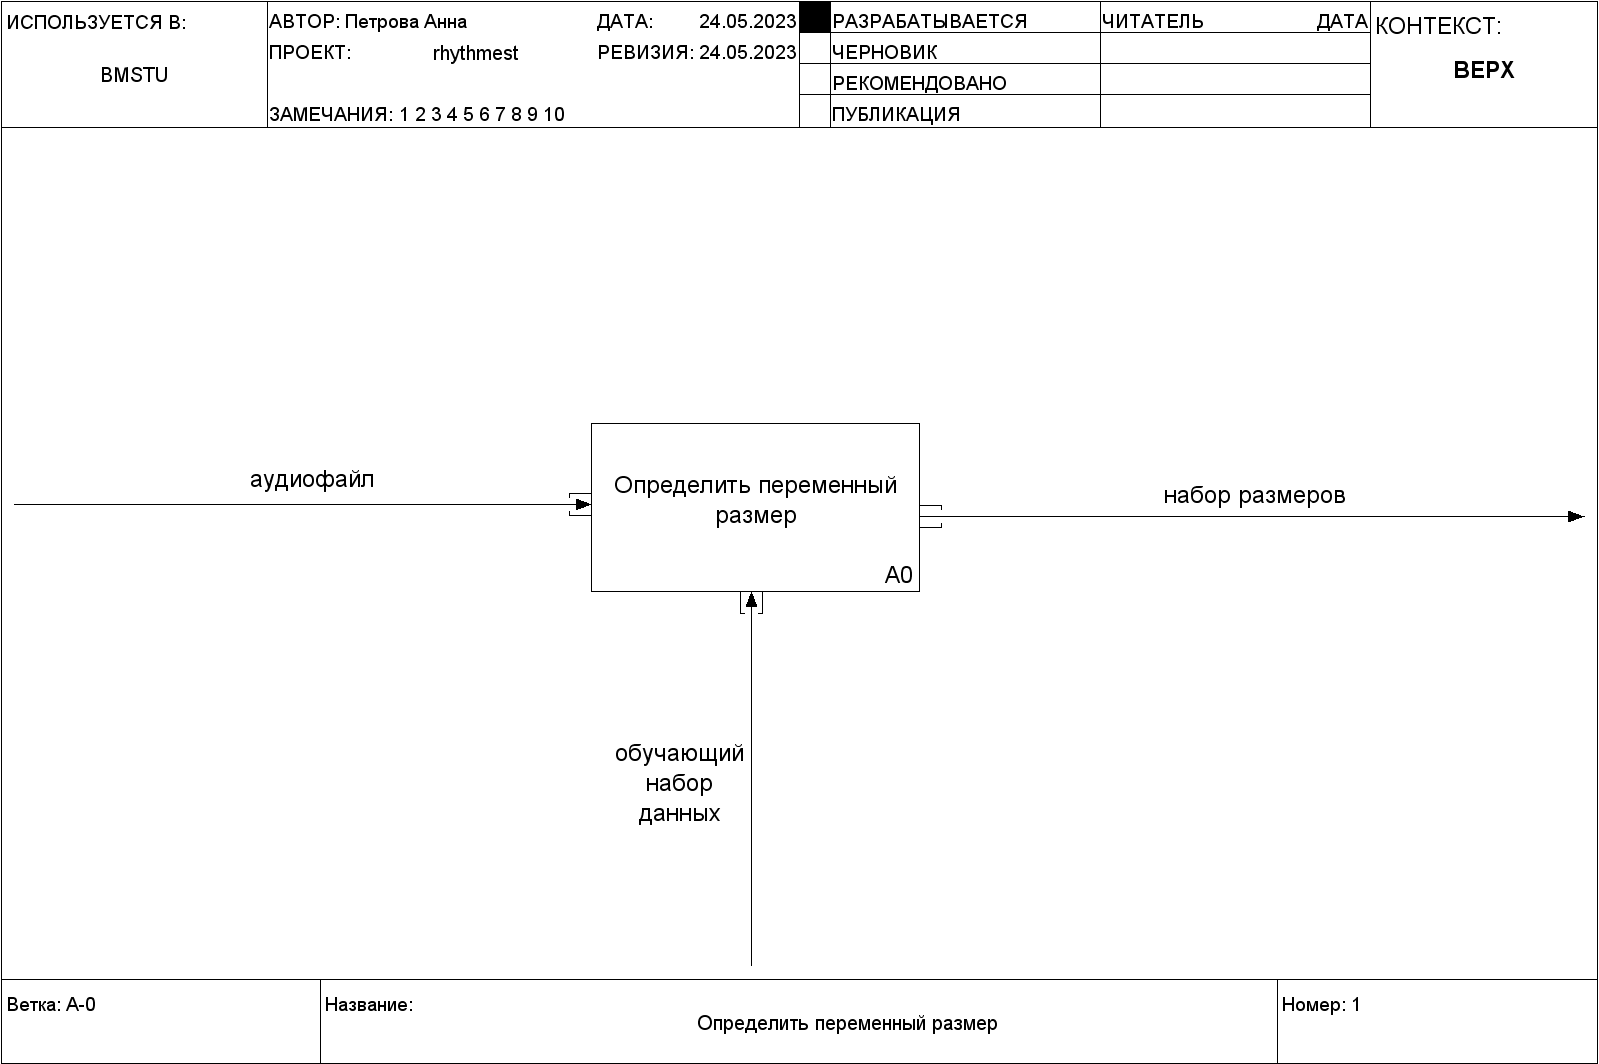
\includegraphics[scale=0.3]{inc/img/rhythm_idef/01_A-0.png}
	\caption{IDEF0 нулевого уровня}
	\label{img:rhythm_0}
\end{figure}

\begin{figure}[h]
	\centering
	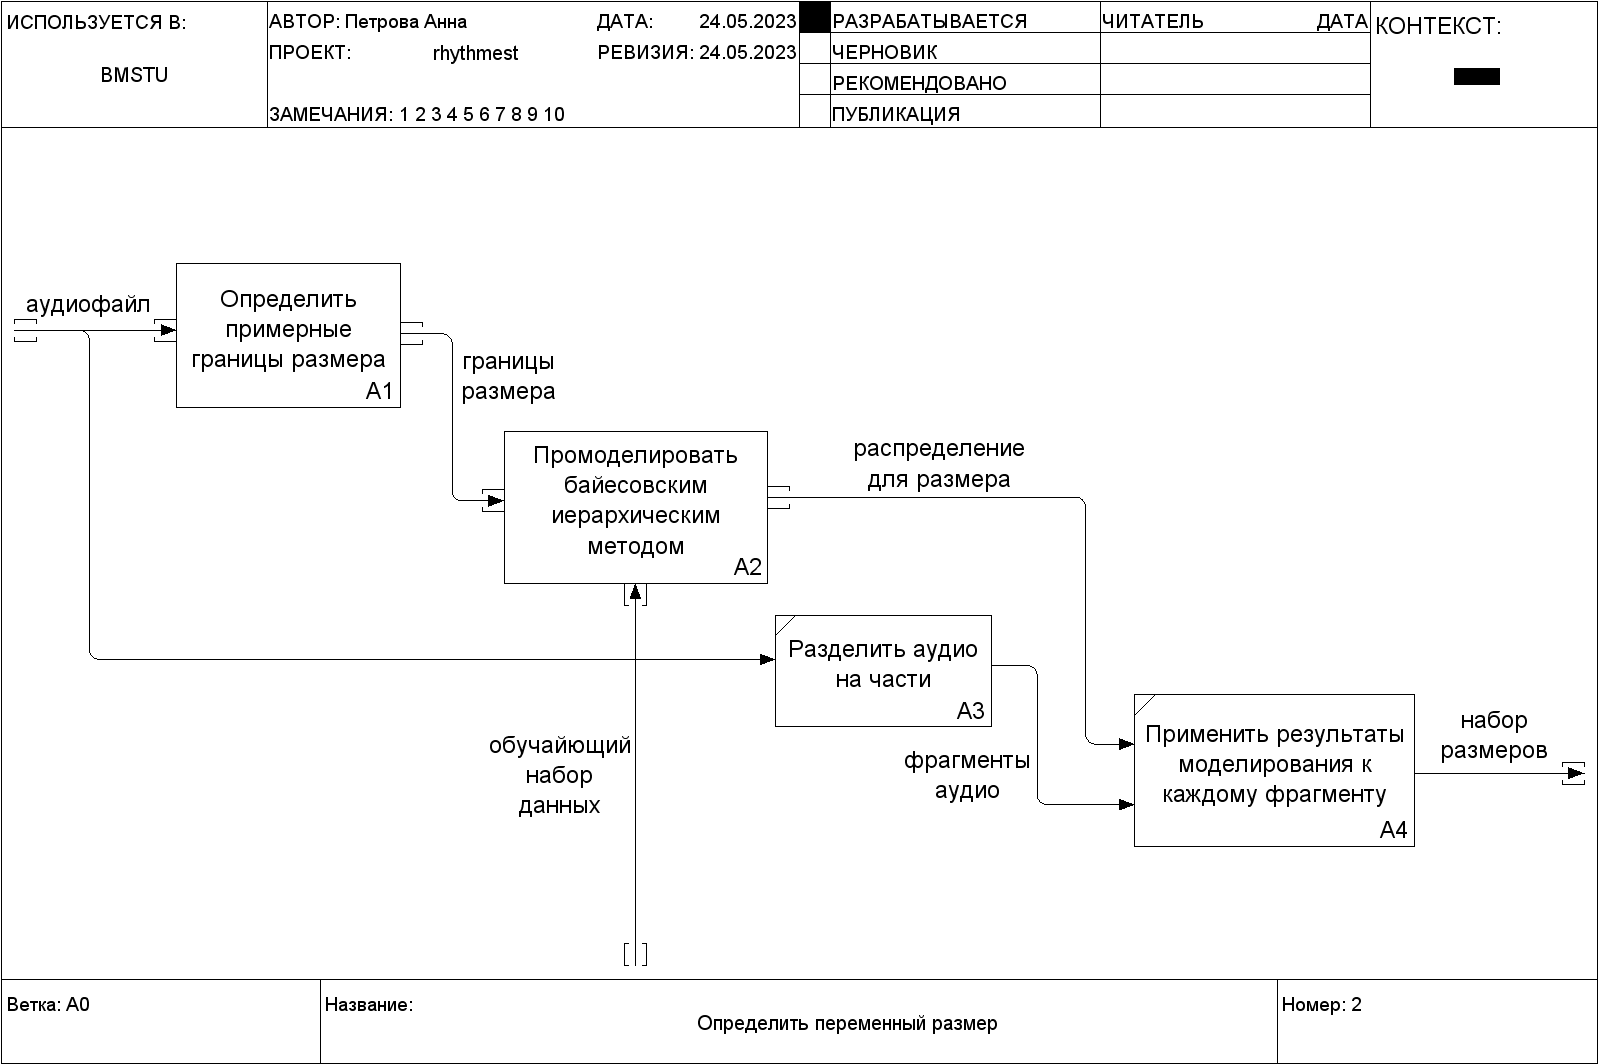
\includegraphics[scale=0.25]{inc/img/rhythm_idef/02_A0.png}
	\caption{Определение переменного ритма}
	\label{img:rhythm_1}
\end{figure}

\begin{figure}[h]
	\centering
	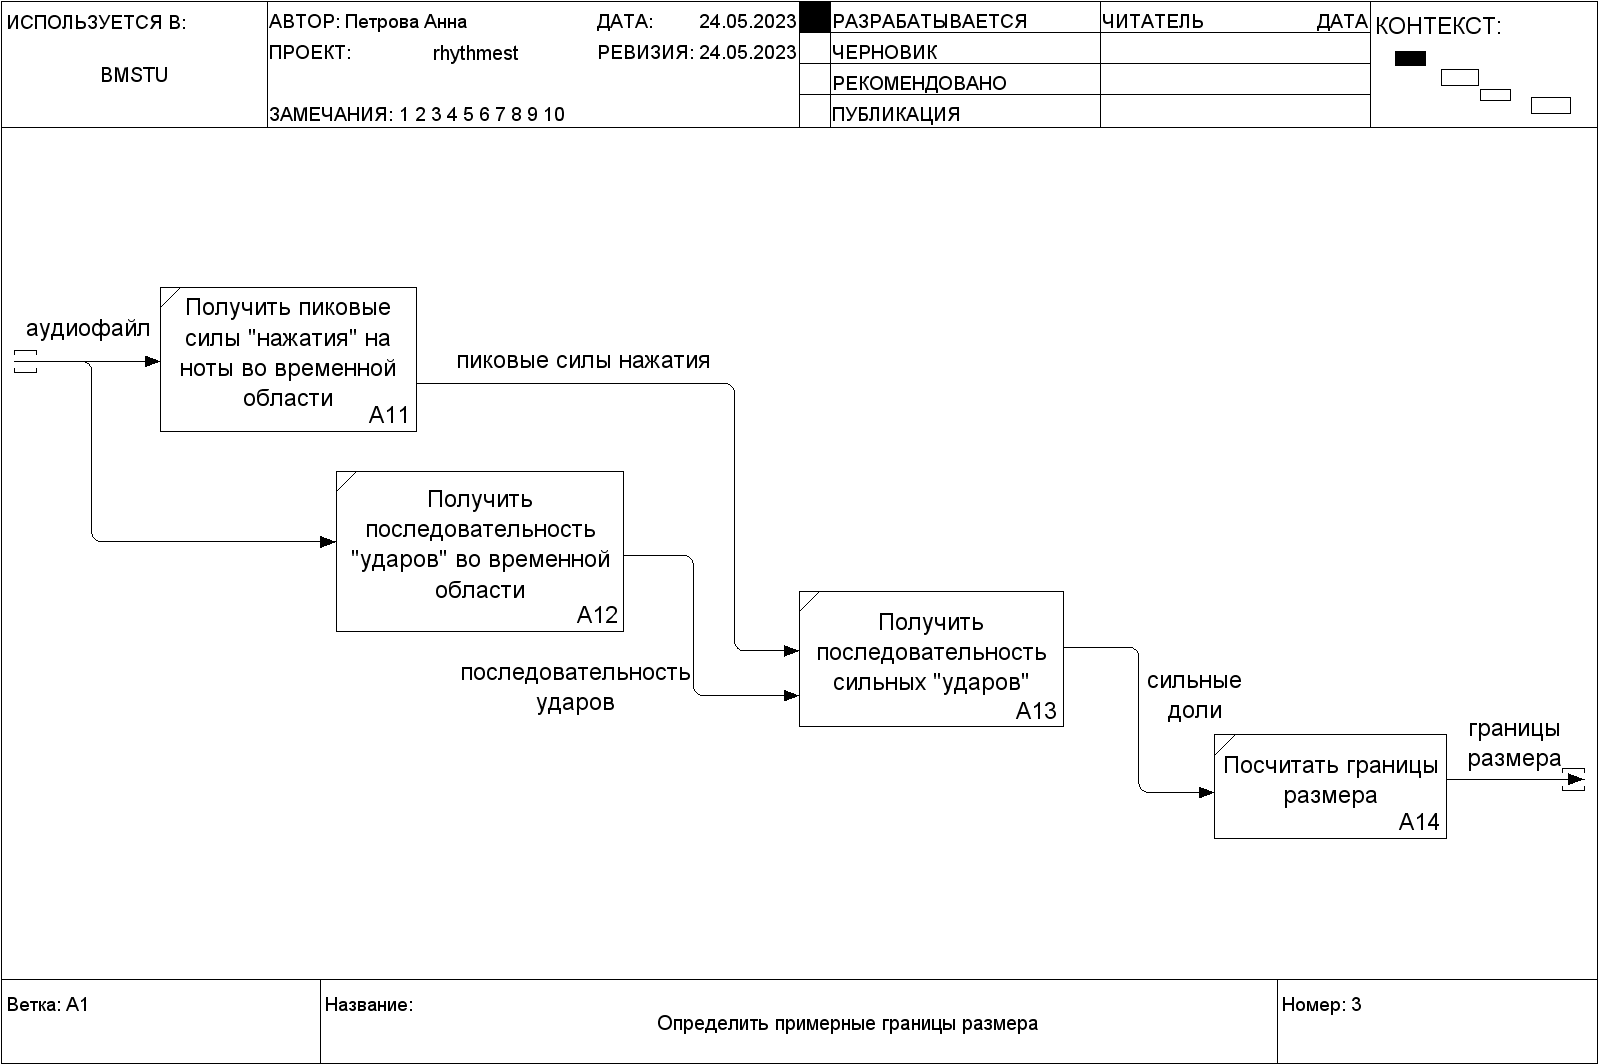
\includegraphics[scale=0.25]{inc/img/rhythm_idef/03_A1.png}
	\caption{Определение границ размера}
	\label{img:rhythm_2}
\end{figure}

\begin{figure}[h]
	\centering
	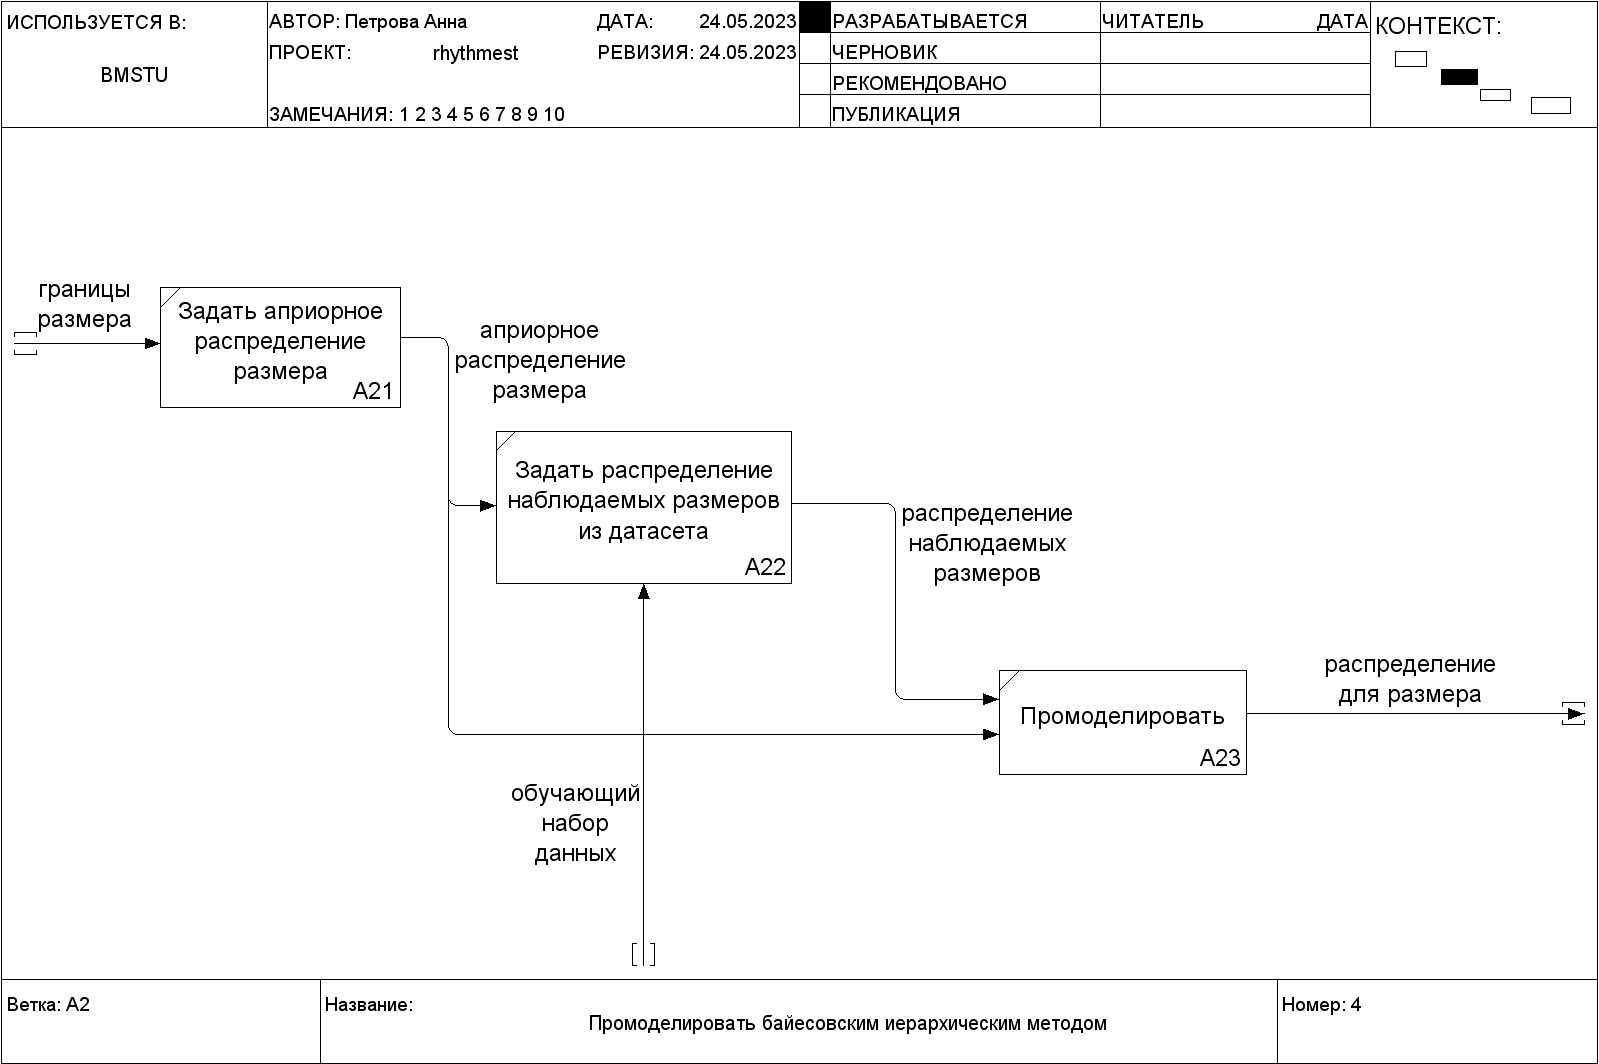
\includegraphics[scale=0.3]{inc/img/rhythm_idef/04_A2.png}
	\caption{Байесовское моделирование}
	\label{img:rhythm_3}
\end{figure}

\clearpage

\subsection{Исходные коды и интерфейс}

В листингах ниже представлены реализации байесовских иерархических моделей для определения темпа и ритма (тактового размера) музыки. Для разработки моделей исполльзовалась библиотека PyMC3~\cite{pymc3_docs}, а для работы с аудио -- библиотека librosa~\cite{librosa}.

\begin{lstlisting}[label={lst:bpmmodel}, caption={реализация байесовской модели для определения темпа}, language=python]
	def bpm_model(min_bpm: int, max_bpm: int, bpm_dataset, genre_dataset, genres_ints, progress):
		with pm.Model() as model:
			# hyperpriors (lvl 1)
			tempo = pm.Uniform('tempo', lower=min_bpm, upper=max_bpm)
			progress.setValue(20)
			mu = (min_bpm + max_bpm) / 2.0
			sigma = (max_bpm - min_bpm) / 12.0
			genre_coef = pm.Normal('genre_coef', mu=0, sd=1, shape=len(genre_dataset.unique()))
			progress.setValue(40)
	
			# prior (lvl 2)
			bpm_est = mu + genre_coef[genres_ints] * sigma
			progress.setValue(60)
	
			# likelihood (lvl 3)
			bpm_obs = pm.Normal('bpm_obs', mu=bpm_est, sd=sigma, observed=bpm_dataset)
			progress.setValue(80)
	
			# get the samples
			trace = pm.sample(1000, tune=500, chains=2, cores=1)
			progress.setValue(100)
	
		return trace
\end{lstlisting}

\begin{lstlisting}[label={lst:measuremodel}, caption={реализация байесовской модели для определения ритма}, language=python]
	def rhythm_model(measure_min, measure_max, rhythm_dataset, progress):
		with pm.Model() as model:
			# prior
			measure = pm.Uniform('measure', lower=measure_min, upper=measure_max)
			progress.setValue(20)
			mu = (measure_min + measure_max) / 2.0
			progress.setValue(40)
			sigma = (measure_max - measure_min) / 12.0
			progress.setValue(60)
	
			# likelihood
			measure_obs = pm.Normal('measure_obs', mu=mu, sd=sigma, observed=rhythm_dataset)
			progress.setValue(80)
	
			trace = pm.sample(1000, tune=1000, chains=2)
			progress.setValue(100)
	
		return trace
\end{lstlisting}

На рисунке~\ref{img:gui} представлен интерфейс разработанного приложения~\cite{pyqt}.

\begin{figure}[h]
	\centering
	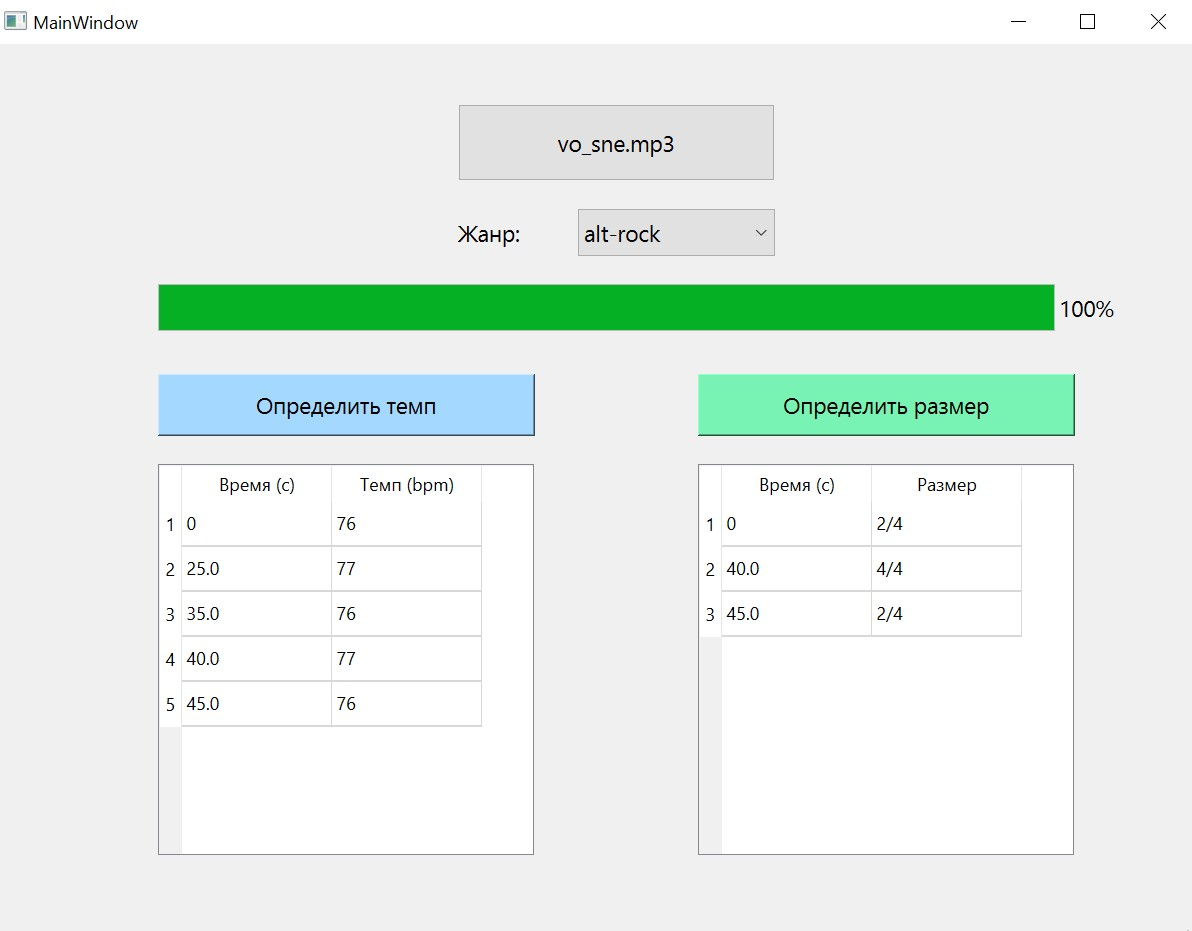
\includegraphics[scale=0.7]{inc/img/gui.jpg}
	\caption{Интерфейс приложения}
	\label{img:gui}
\end{figure}
